\documentclass{exam}
\usepackage{../../mypackages}
\usepackage{../../macros}

\title{Interro N°2 - Atome et Réactions Chimiques}
\author{N. Bancel}
\date{Novembre 2024}

\begin{document}

\textbf{Collège Lycée Suger}
\hfill
\textbf{Physique-Chimie} \\

\textbf{Année 2024-2025}
\hfill
\textbf{3ème Cambridge International} \par

{\let\newpage\relax\maketitle}

\begin{center}
\textbf{\textcolor{red}{Durée : 45 minutes. La calculatrice n'est pas autorisée}} \\
\textbf{\textcolor{red}{Une réponse donnée sans justification sera considérée comme fausse.}} \\
Cette interrogation contient \numquestions\ questions, sur \numpages\ pages et est notée sur 10. 

\end{center}

\section*{Partie 1 : Structure de l'Atome et Propriétés (5 points)}

\begin{questions}
  \question[1] Donnez la signification de $A$, $X$, et $Z$ dans la notation symbolique d'un atome.

\begin{figure}[H]
    \centering
    
\includegraphics[width=0.2\linewidth]{interro2_01.jpg}
    \caption{Structure simplifiée d'un atome}
\end{figure} 

  \question[1.5] Compléter la figure ci-dessous. Il est obligatoire de donner une justification de la méthode en amont (pas besoin de la ré expliquer à chaque fois). Aucun point ne sera attribué si aucune justification n'est apportée.

  \begin{figure}[H]
    \centering
    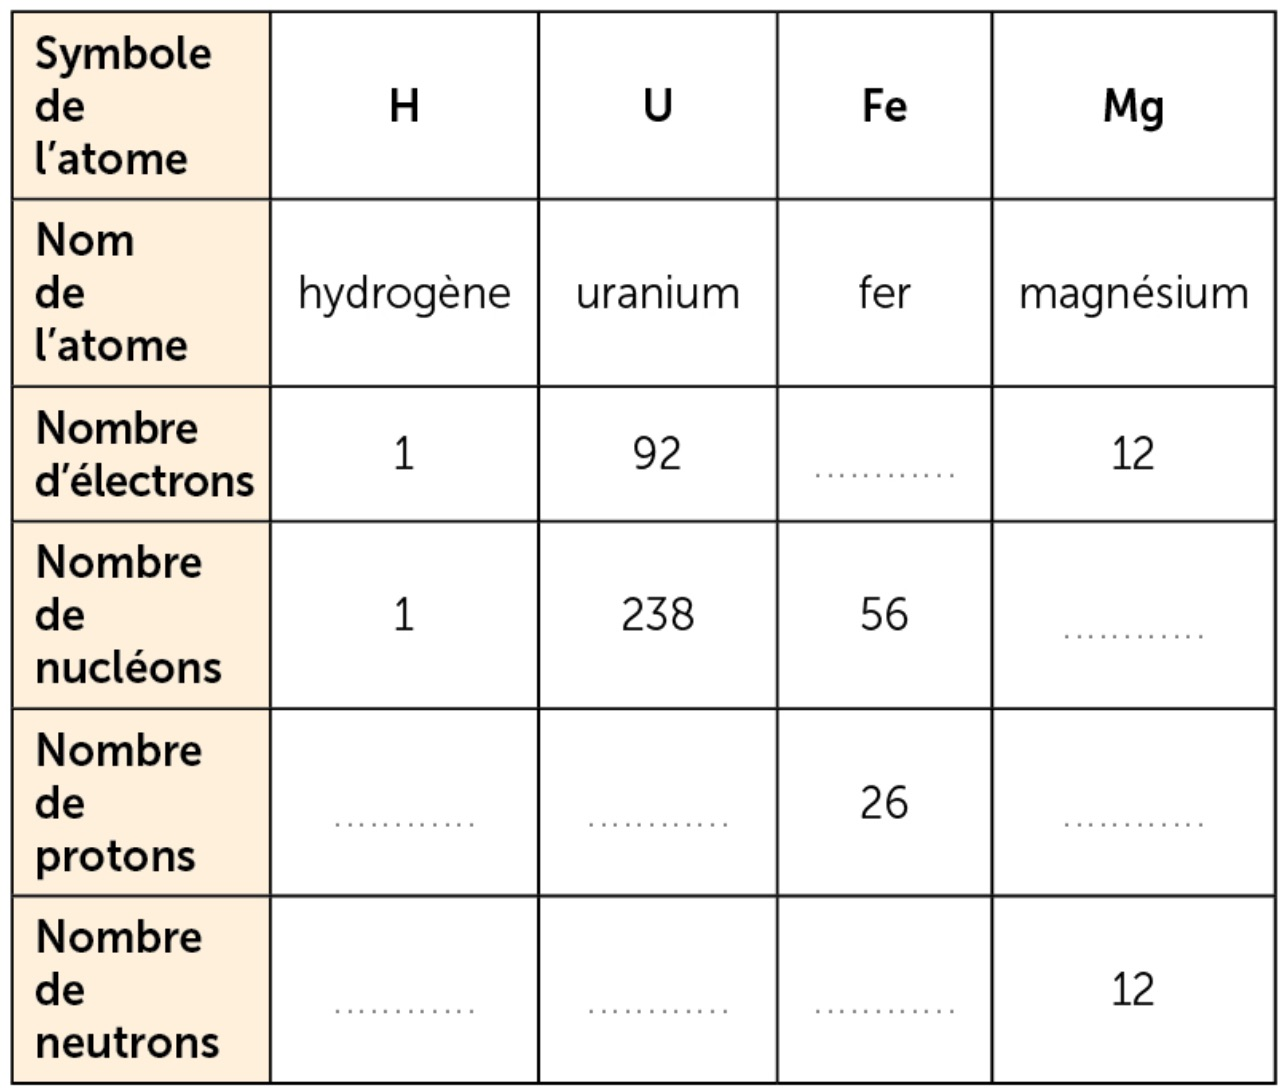
\includegraphics[width=0.6\linewidth]{interro2_02.jpg}
    \caption{Composants de l'atome}
\end{figure} 

  \question[0.5] Expliquez pourquoi un atome est neutre électriquement.

  \question[1.5] Basé sur les informations ci-dessous, de combien de fois la masse d’un nucléon est-elle supérieure à celle d’un électron ? 

  \begin{center}
  \begin{tabular}{SS}
    \toprule
    {Constituant} & {Masse (en \si{kg})} \\
    \midrule
    {Electron} & {\(9.1 \times 10^{-31}\)} \\
    {Nucléon (Proton et Neutron)} & {\(1.7 \times 10^{-27}\)} \\
    \bottomrule
  \end{tabular}
\end{center}
  
  \question[0.5] Expliquer la différence entre un atome et une molécule, et donnez un exemple de chaque.

\end{questions}

\section*{Partie 2 : Réactions chimiques (5 points)}

\begin{questions}

  \question[0.75] Donnez les formules des molécules suivantes :
  \begin{itemize}[noitemsep]
    \item Dioxygène
    \item Dioxyde de carbone
    \item Eau
  \end{itemize}

  \question[1] La paille de fer (\ce{Fe}) brûle facilement dans l'air (au contact du dioxygène \ce{O2}). Il se forme alors de petites boules d'oxyde magnétique de fer, de formule \ce{Fe3O4}. 
  \begin{parts}
    \part[0.25] Quelle est la constitution en atomes de l'oxyde magnétique de fer ? Préciser le nom et le nombre de chaque type d'atomes.
    \part[0.25] Ecrire en toutes lettres la réaction chimique traduisant la transformation entre le fer et le dioxygène de l'air.
    \part[0.5] Ecrire et équilibrer l'équation chimique qui a lieu.
\end{parts}
  
  \question[1]  Adam réalise l'expérience schématisée ci-dessous

  \begin{figure}[H]
    \centering
    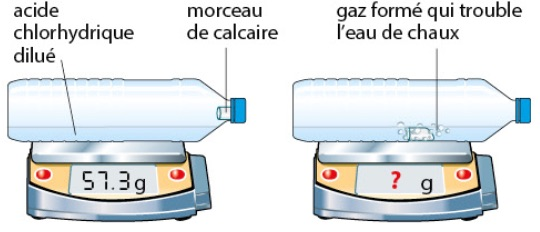
\includegraphics[width=0.6\linewidth]{interro2_03.jpg}
    \caption{Structure simplifiée d'un atome}
\end{figure} 

  \begin{parts}
    \part[0.25] Quels sont les réactifs ?
    \part[0.25] Quelle est la masse de ces réactifs ?
    \part[0.5] Qu'indique la balance de droite ? Pourquoi ?
\end{parts}


  \question[1.5] Les équations chimiques ci-dessous sont-elles équilibrées ? Justifier pourquoi. Si elles ne le sont pas, les équilibrer.
  \begin{parts}
    \part[0.5] \ce{H2O -> H2 + O2}
    \part[0.5] \ce{C + O2 -> CO}
    \part[0.5] \ce{CH4 + O2 -> CO2 + H2O}
\end{parts}

\question[0.75] Quelle est la formule de la réaction chimique ci-dessous ? Est-elle équilibrée ?

\begin{figure}[H]
  \centering
  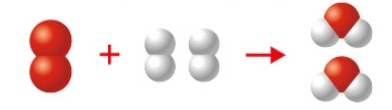
\includegraphics[width=0.6\linewidth]{interro2_04.jpg}
  \caption{Réaction chimique}
\end{figure} 


\end{questions}

\section*{Aide au calcul}

Ces calculs (pas tous) peuvent aider à la résolution des exercices :
\begin{itemize}
  \item $238 + 92 = 330$
  \item $92 + 146 = 238$
  \item $\frac{9.1}{1.7} \approx 5.353$
  \item $\frac{1.7}{9.1} \approx 0.187$
  \item $1.7 + 9.1 = 10.8$
  \item En considérant $a$ et $b$ des nombres entiers : 
  \begin{itemize}
    \item $\frac{10^a}{10^b} = 10^{a-b}$
    \item $10^a \times 10^b = 10^{a+b}$ 
  \end{itemize}
\end{itemize}

\end{document}
